\documentclass[tikz]{standalone}
\begin{document}
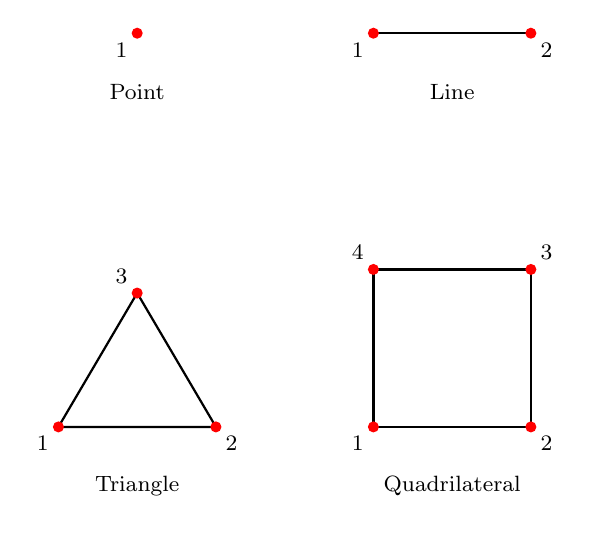
\begin{tikzpicture}
  [
    font=\footnotesize,
    edg/.style={thick},
    vtx/.style={red}
  ]
  \coordinate [label=below left:{$1$}]  (P1) at (1.0, 5.0);
  \coordinate [label=below left:{$1$}]  (L1) at (4.0, 5.0);
  \coordinate [label=below right:{$2$}] (L2) at (6.0, 5.0);
  \coordinate [label=below left:{$1$}]  (T1) at (0.0, 0.0);
  \coordinate [label=below right:{$2$}] (T2) at (2.0, 0.0);
  \coordinate [label=above left:{$3$}]  (T3) at (1.0, 1.7);
  \coordinate [label=below left:{$1$}]  (Q1) at (4.0, 0.0);
  \coordinate [label=below right:{$2$}] (Q2) at (6.0, 0.0);
  \coordinate [label=above right:{$3$}] (Q3) at (6.0, 2.0);
  \coordinate [label=above left:{$4$}]  (Q4) at (4.0, 2.0);
  \draw (P1);
  \draw [edg] (L1) -- (L2);
  \draw [edg] (T1) -- (T2) -- (T3) -- cycle;
  \draw [edg] (Q1) -- (Q2) -- (Q3) -- (Q4) -- cycle;
  \foreach \point in {P1, L1, L2, T1, T2, T3, Q1, Q2, Q3, Q4}
    \fill [vtx] (\point) circle (2pt);
  \node at (1.0,  4.25) {Point};
  \node at (5.0,  4.25) {Line};
  \node at (1.0, -0.75) {Triangle};
  \node at (5.0, -0.75) {Quadrilateral};
\end{tikzpicture}
\end{document}
